\documentclass[\main.tex]{subfiles}

\chapter{Estado Atual da Aplicação}
\begin{singlespace}
\minitoc
\end{singlespace}
\vspace{40pt}

Atualmente, o componente de gestão de utilizadores da aplicação está totalmente funcional, com o registo
e o login de utilizadores. Estão a ser corrigidos alguns precalços ocorridos no desenvolvimento da gestão
de sessões de utilizadores, para que apenas utilizadores registados e logados no sistema possam jogar.\par
Na figura 4.1 e 4.2 estão representados o componente de login e registo de um utilizador, respetivamente.\par

\begin{figure}[h!]
\centering
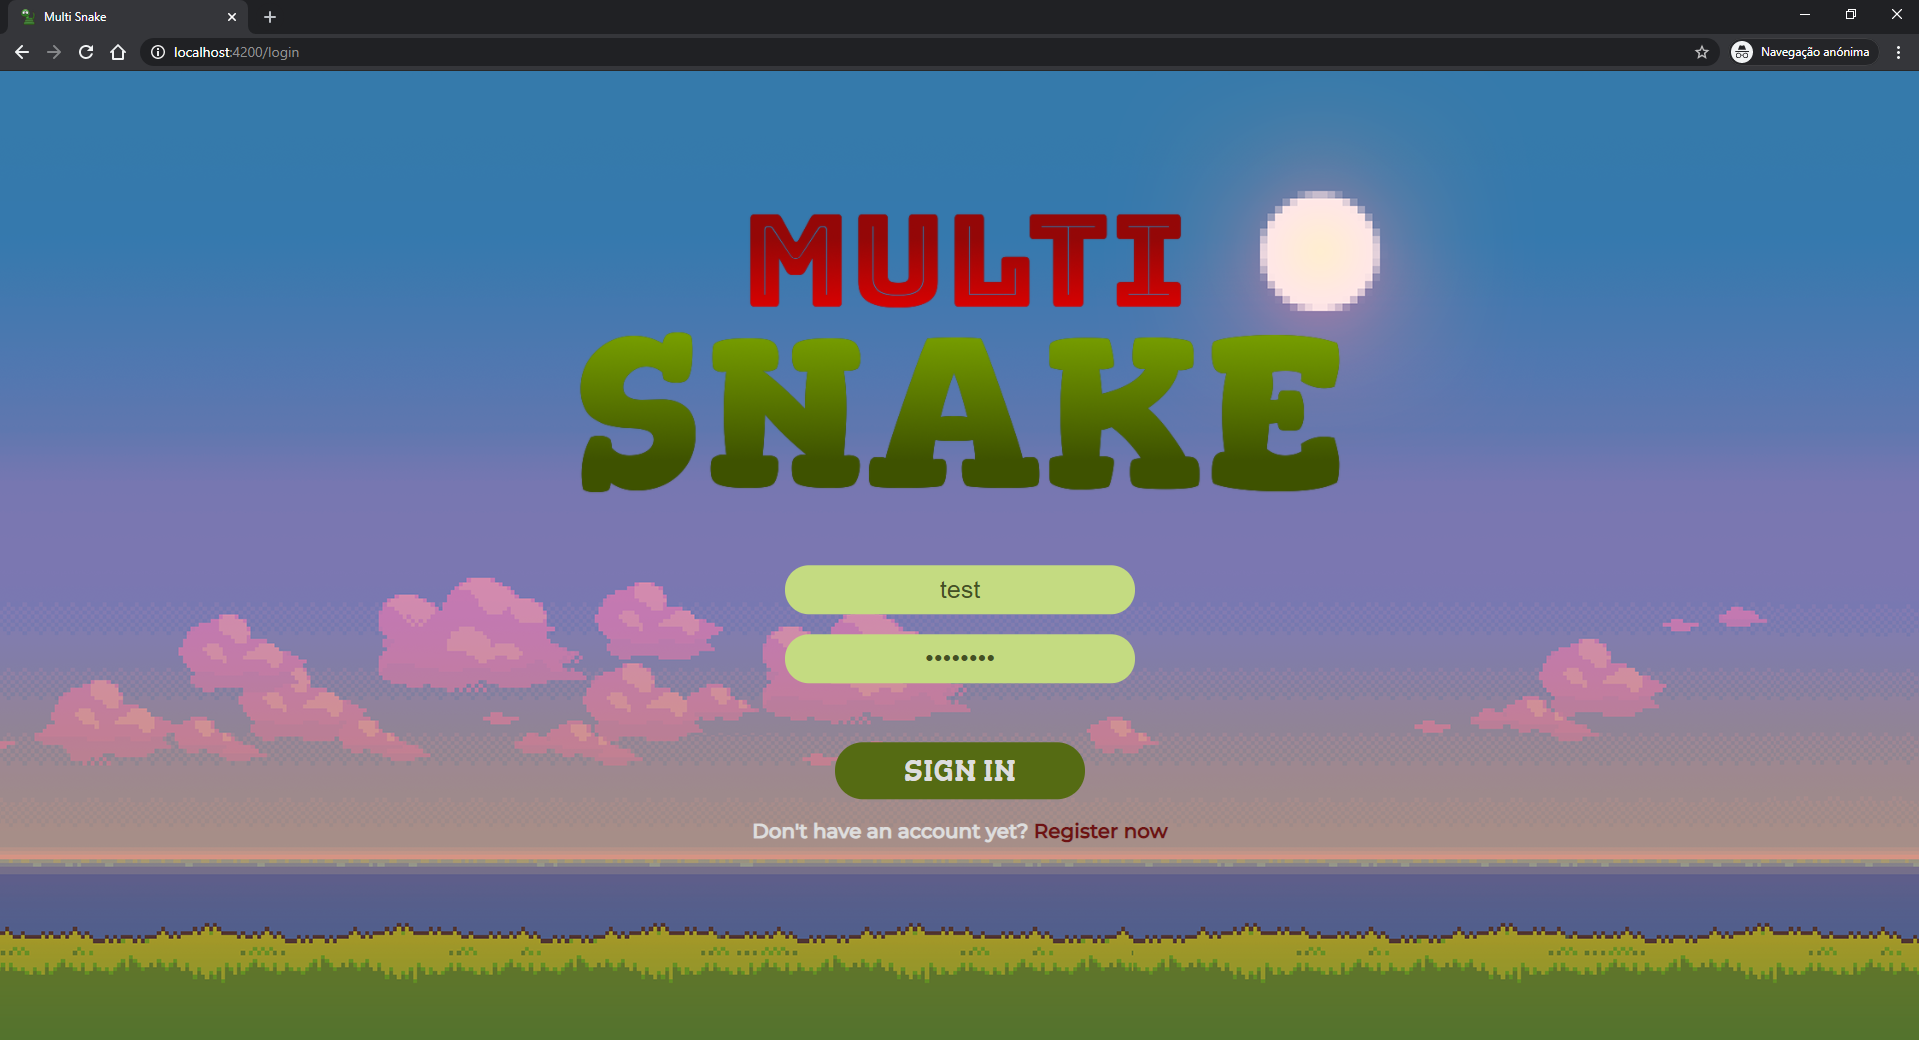
\includegraphics[width=\linewidth]{../private_assets/Login.png}
\caption{Componente de login de utilizadores}
\end{figure}

\newpage

\begin{figure}[h!]
\centering
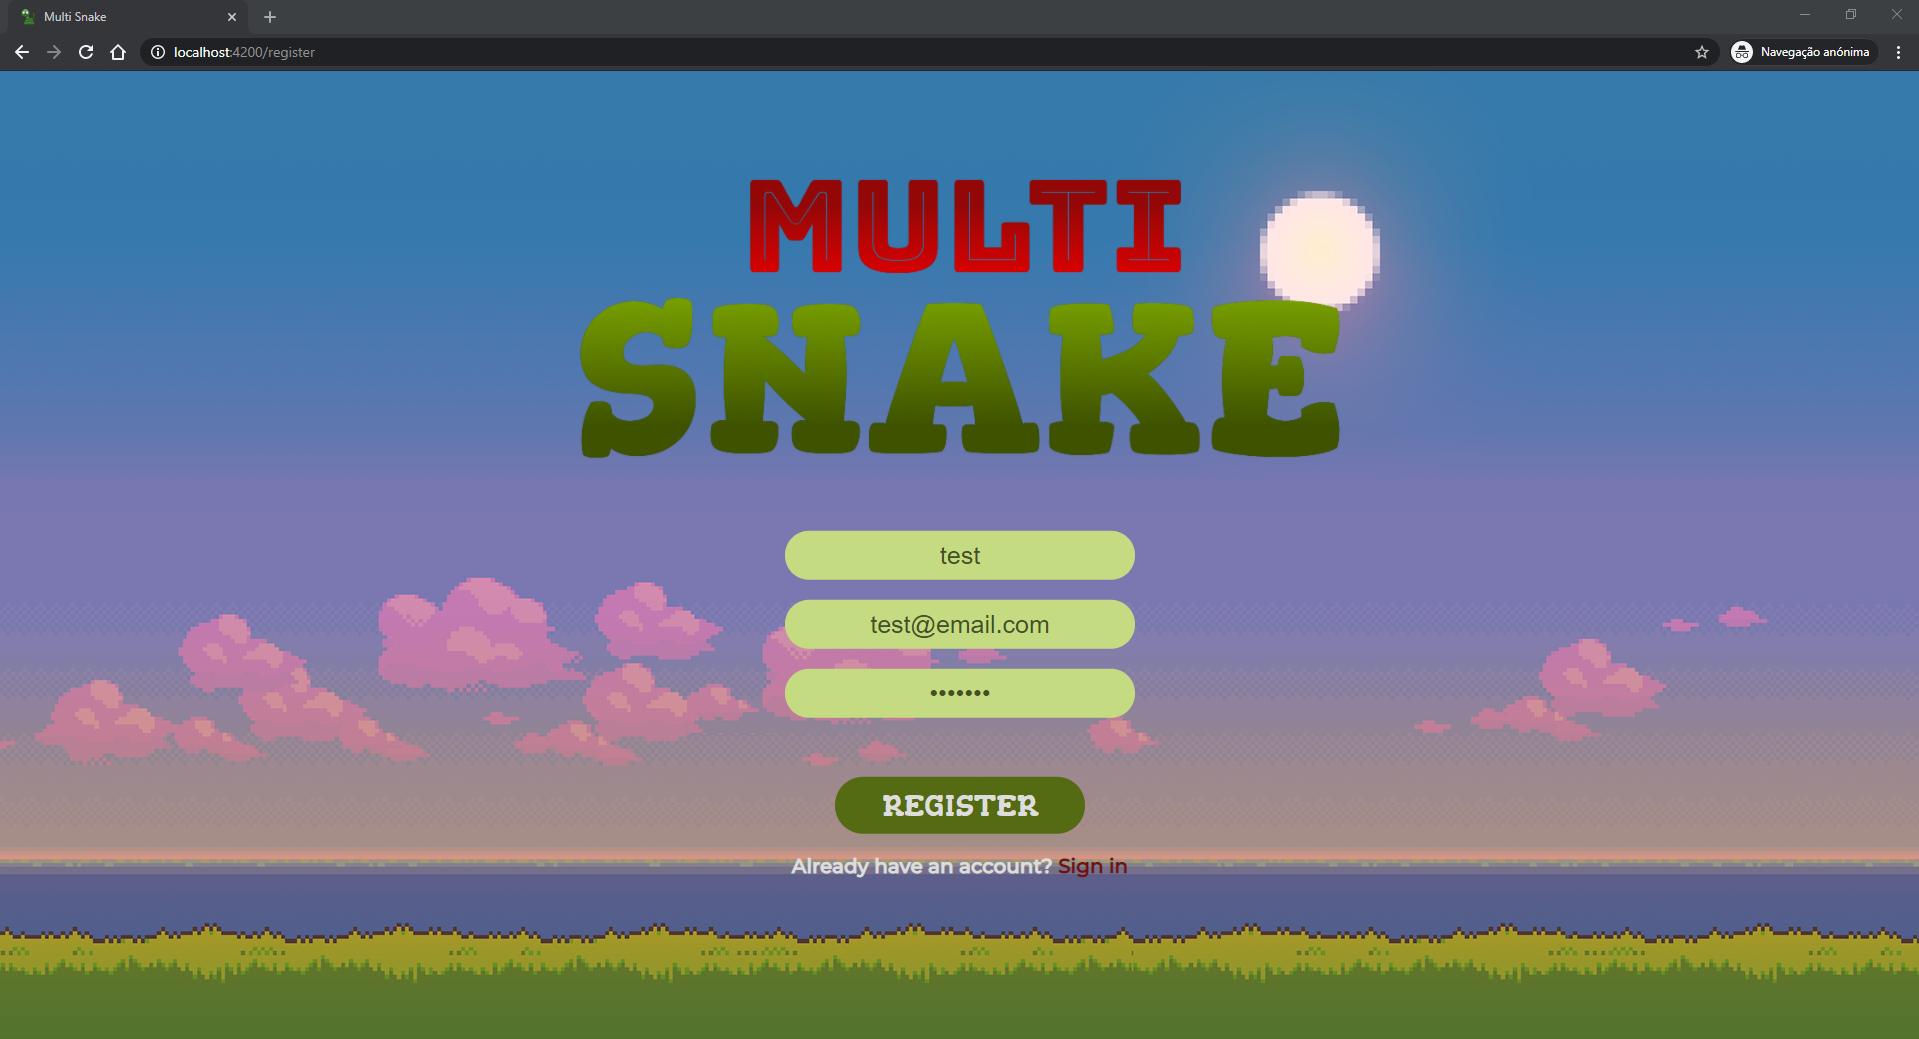
\includegraphics[width=\linewidth]{../private_assets/Register.png}
\caption{Componente de registo de utilizadores}
\end{figure}

\vspace{40pt}

Em desenvolvimento está também a página pessoal de cada utilizador, dentro da qual foi realizada uma
versão singleplayer do jogo da cobra, para servir de apoio e modelo para o desenvolvimento do modo
multiplayer. A figura 4.3 demonstra uma fase bastante primordial da página privada do utilizador com a
versão do jogo para um jogador.\par

\begin{figure}[h!]
\centering
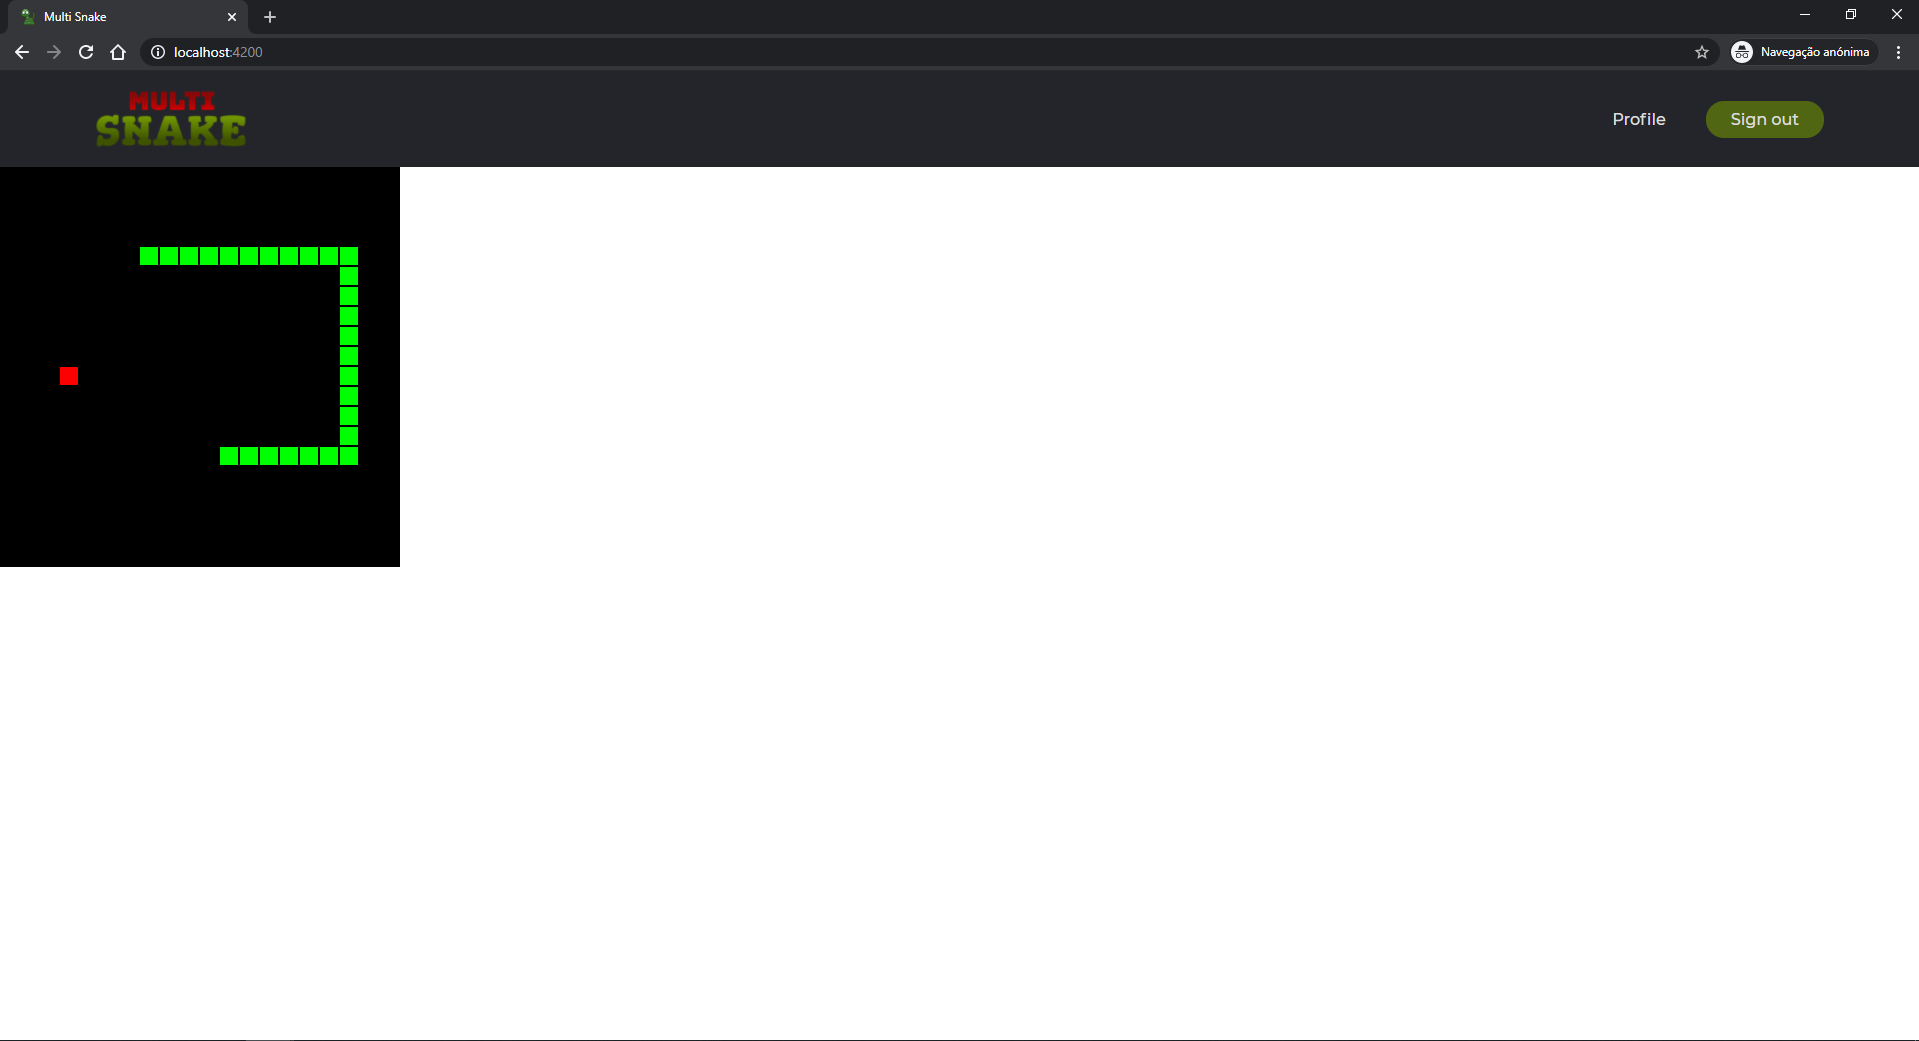
\includegraphics[width=\linewidth]{../private_assets/SinglePlayer.png}
\caption{Página privada de um utilizador com a versão singleplayer do jogo da cobra}
\end{figure}